\chapter{Analisi dei requisiti}
\label{cap:analisi-requisiti}

\intro{Di seguito viene riportata l'Analisi dei Requisiti del prodotto software, partendo dai casi d'uso e poi a seguire il tracciamento dei requisiti concordati con il proponente.}\\

\section{Casi d'uso}

Per lo studio dei casi di utilizzo del prodotto sono stati creati dei diagrammi.\newline
I diagrammi dei casi d'uso (in inglese \emph{Use Case Diagram}) sono diagrammi di tipo \gls{uml} dedicati alla descrizione delle funzioni o servizi offerti da un sistema, così come sono percepiti e utilizzati dagli attori che interagiscono col sistema stesso.\newline
Per convenzione i casi d'uso saranno classificati con questo codice:
\begin{center}
\textbf{UC[codice padre](.[Codice figlio])}
\end{center}
Dove UC indica \emph{Use Case} e i due codici sono:
\begin{itemize}
	\item \textbf{Codice padre} è il codice identificativo numerico del dato caso d’uso;
    \item \textbf{Codice figlio} è il codice identificativo di un eventuale sotto caso d’uso.
\end{itemize}

%Essendo il progetto finalizzato alla creazione di un tool per l'automazione di un processo, le interazioni da parte dell'utilizzatore devono essere ovviamente ridotte allo stretto necessario. Per questo motivo i diagrammi d'uso risultano semplici e in numero ridotto.\newline

%\begin{figure}[!h] 
%    \centering 
%    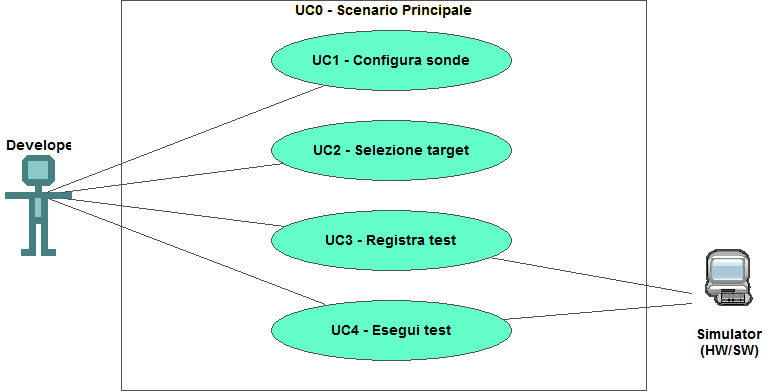
\includegraphics[width=0.9\columnwidth]{usecase/scenario-principale} 
%    \caption{Use Case - UC0: Scenario principale}
%\end{figure}
%
%\begin{usecase}{0}{Scenario principale}
%\usecaseactors{Sviluppatore applicativi}
%\usecasepre{Lo sviluppatore è entrato nel plug-in di simulazione all'interno dell'IDE}
%\usecasedesc{La finestra di simulazione mette a disposizione i comandi per configurare, registrare o eseguire un test}
%\usecasepost{Il sistema è pronto per permettere una nuova interazione}
%\label{uc:scenario-principale}
%\end{usecase}

\subsection{Attori}

Gli attori principali che andranno ad interagire con l'applicazione sono i seguenti:
\begin{itemize}
    \item \textbf{Utente non autenticato}
    \item \textbf{Utente}
    \item \textbf{Amministratore}
\end{itemize}
Nell'analisi è stato identificato un quarto attore, ovvero \textbf{ChatGPT}, in quanto tra i requisiti desiderabili era prevista l'integrazione dello stesso per consigliare le ricette, ma alla fine dello stage questa integrazione non è stata svolta, preferendo dare priorità ai requisiti obbligatori e al funzionamento vero e proprio dell'applicazione.

\newpage

\subsection{Diagrammi e descrizione}

Di seguito sono riportati i casi d'uso nel dettaglio, analizzando per ogni caso gli attori principali, la descrizione, la precondizione e la postcondizione; gli ultimi due riportano lo stato dell'applicazione, o lo stato di un attore, rispettivamente prima e dopo l'esecuzione del caso d'uso studiato.\newline
\newline
Gli \emph{use case} sono stati divisi in base alle azioni che devono essere svolte in ogni schermata dell'app (Home, Spese, Menu, Utente e Impostazioni), viene fatta eccezione per gli \emph{use case} riguardanti il Primo Accesso e a ChatGPT perchè possono essere gestiti in schermate distinte o integrate nelle schermate principali.\newline
Sono stati analizzati in modo distinto anche i sottocasi d'uso; per gli \emph{use case} padre si elenca la generalizzazione dei propri sotto casi.\newline

\begin{figure}[!h] 
    \centering 
    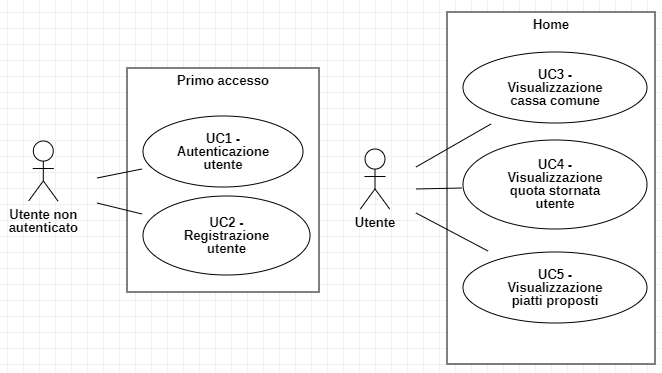
\includegraphics[width=0.9\columnwidth]{usecase/usecase-1} 
    \caption{Use Case - Primo accesso e Home}
    \label{fig:uc-accessoehome}
\end{figure}

\begin{usecase}{1}{Autenticazione utente - Figura \ref{fig:uc-accessoehome}}
    \usecaseactors{Utente non autenticato}
    \usecasepre{L'utente non ha effettuato l'autenticazione}
    \usecasedesc{L'utente inserisce la propria mail e la propria password per effettuare l'accesso}
    \usecasepost{L'utente è stato autenticato}
    \label{uc:autenticazione-utente}
\end{usecase}

\begin{usecase}{2}{Registrazione utente - Figura \ref{fig:uc-accessoehome}} 
    \usecaseactors{Utente non autenticato}
    \usecasepre{L'utente non è registrato nel database}
    \usecasedesc{L'utente inserisce i propri dati per registrarsi nel database}
    \usecasepost{L'utente è registrato nel database}
    \label{uc:registrazione-utente}
\end{usecase}

\begin{usecase}{3}{Visualizzazione \emph{\gls{cassacomuneg}} - Figura \ref{fig:uc-accessoehome}}
    \usecaseactors{Utente}
    \usecasepre{La \emph{\gls{cassacomuneg}} non è visibile}
    \usecasedesc{L'utente entra nell'app per visualizzare la \emph{\gls{cassacomuneg}}}
    \usecasepost{L'utente visualizza la \emph{\gls{cassacomuneg}}}
    \label{uc:visualizza-casacomune}
\end{usecase}

\begin{usecase}{4}{Visualizzazione \emph{\gls{quotastornatag}} utente - Figura \ref{fig:uc-accessoehome}}
    \usecaseactors{Utente}
    \usecasepre{La \emph{\gls{quotastornatag}} dell'utente non è visibile}
    \usecasedesc{L'utente entra nell'app per visualizzare la propria \emph{\gls{quotastornatag}}}
    \usecasepost{L'utente visualizza la propria \emph{\gls{quotastornatag}}}
    \label{uc:visualizza-quotastornata}
\end{usecase}

\begin{usecase}{5}{Visualizzazione piatti proposti - Figura \ref{fig:uc-accessoehome}}
    \usecaseactors{Utente}
    \usecasepre{La lista dei piatti proposti del giorno non è visibile}
    \usecasedesc{L'utente entra nell'app per visualizzare i piatti proposti del giorno}
    \usecasepost{L'utente visualizza la lista dei piatti proposti del giorno}
    \label{uc:visualizza-piattiproposti}
\end{usecase}

\begin{figure}[!h] 
    \centering 
    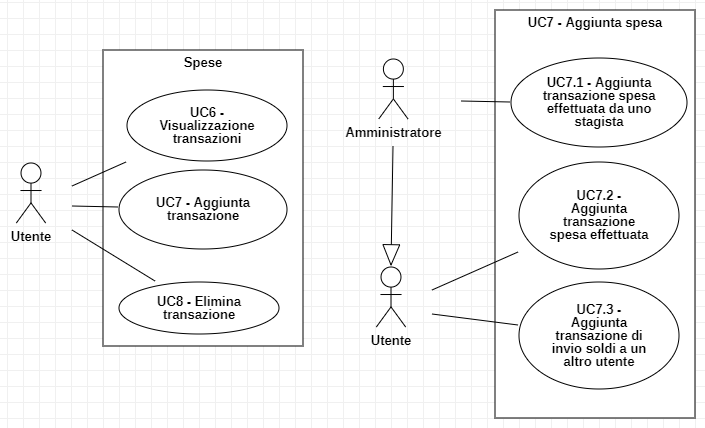
\includegraphics[width=1.0\columnwidth]{usecase/usecase-2} 
    \caption{Use Case - Spese e UC7}
    \label{fig:uc-spese}
\end{figure}

\newpage

\begin{usecase}{6}{Visualizzazione transazioni - Figura \ref{fig:uc-spese}}
    \usecaseactors{Utente}
    \usecasepre{La lista delle transazioni non è visibile}
    \usecasedesc{L'utente entra nell'app per visualizzare la lista delle transazioni}
    \usecasepost{L'utente visualizza la lista delle transazioni}
    \label{uc:visualizza-transazioni}
\end{usecase}

\begin{usecase}{7}{Aggiunta transazione - Figura \ref{fig:uc-spese}}
    \usecaseactors{Utente}
    \usecasepre{La transazione non è presente nel database e non è visibile nella lista delle transazioni}
    \usecasedesc{L'utente inserisce i dati della transazione interessata e la salva nel database}
    \usecasepost{La transazione è presente nel database e visibile nella lista delle transazioni}
    \label{uc:aggiungi-transazione}
\end{usecase}

\noindent \textbf{Generalizzazioni:}
\begin{itemize}
    \item \ref{uc:aggiungi-spesastagista} - Aggiunta transazione spesa effettuata da uno stagista
    \item \ref{uc:aggiungi-spesa} - Aggiunta transazione spesa effettuata
    \item \ref{uc:aggiungi-inviosoldi} - Aggiunta transazione di invio soldi a un altro utente
\end{itemize}

\begin{usecase}{7.1}{Aggiunta transazione spesa effettuata da uno stagista - Figura \ref{fig:uc-spese}}
    \usecaseactors{Amministratore}
    \usecasepre{La spesa effettuata da uno stagista non è presente nel database e non è visibile nella lista delle transazioni}
    \usecasedesc{L'amministratore inserisce i dati della spesa effettuata da uno stagista e la salva nel database}
    \usecasepost{La spesa effettuata da uno stagista è presente nel database e visibile nella lista delle transazioni}
    \label{uc:aggiungi-spesastagista}
\end{usecase}

\begin{usecase}{7.2}{Aggiunta transazione spesa effettuata - Figura \ref{fig:uc-spese}}
    \usecaseactors{Utente}
    \usecasepre{La spesa effettuata dall'utente non è presente nel database e non è visibile nella lista delle transazioni}
    \usecasedesc{L'utente inserisce i dati della spesa effettuata e la salva nel database}
    \usecasepost{La spesa dell'utente è presente nel database e visibile nella lista delle transazioni}
    \label{uc:aggiungi-spesa}
\end{usecase}

\newpage

\begin{usecase}{7.3}{Aggiunta transazione di invio soldi a un altro utente - Figura \ref{fig:uc-spese}}
    \usecaseactors{Utente}
    \usecasepre{L'invio dei soldi tra due utenti non è presente nel database e non è visibile nella lista delle transazioni}
    \usecasedesc{L'utente inserisce i dati dell'invio dei soldi a un altro utente e lo salva nel database}
    \usecasepost{L'invio dei soldi tra due utenti è presente nel database e visibile nella lista delle transazioni}
    \label{uc:aggiungi-inviosoldi}
\end{usecase}

\begin{usecase}{8}{Elimina transazione - Figura \ref{fig:uc-spese}}
    \usecaseactors{Utente}
    \usecasepre{La transazione è presente nel database e visibile nella lista delle transazioni}
    \usecasedesc{L'utente elimina la transazione interessata dall'app e viene eliminata dal database}
    \usecasepost{La transazione non è presente nel database e non è visibile nella lista delle transazioni}
    \label{uc:elimina-transazione}
\end{usecase}

\begin{figure}[!h] 
    \centering 
    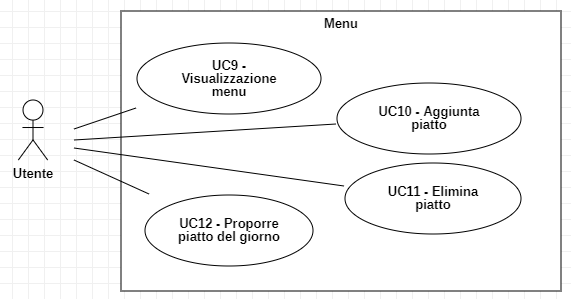
\includegraphics[width=0.8\columnwidth]{usecase/usecase-3} 
    \caption{Use Case - Menu}
    \label{fig:uc-menu}
\end{figure}

\begin{usecase}{9}{Visualizzazione menu - Figura \ref{fig:uc-menu}}
    \usecaseactors{Utente}
    \usecasepre{Il menu non è visibile}
    \usecasedesc{L'utente entra nell'app per visualizzare il menu}
    \usecasepost{L'utente visualizza la lista dei piatti presenti nel menu}
    \label{uc:visualizza-menu}
\end{usecase}

\newpage

\begin{usecase}{10}{Aggiunta piatto - Figura \ref{fig:uc-menu}}
    \usecaseactors{Utente}
    \usecasepre{Il piatto non è presente nel database e non è visibile dal menu}
    \usecasedesc{L'utente inserisce i dati del piatto e lo salva nel database}
    \usecasepost{Il piatto è presente nel database e visibile dal menu}
    \label{uc:aggiungi-piatto}
\end{usecase}

\begin{usecase}{11}{Elimina piatto - Figura \ref{fig:uc-menu}}
    \usecaseactors{Utente}
    \usecasepre{Il piatto è presente nel database e visibile dal menu}
    \usecasedesc{L'utente elimina il piatto interessato dall'app e viene eliminato dal database}
    \usecasepost{Il piatto non è presente nel database e non è visibile dal menu}
    \label{uc:elimina-piatto}
\end{usecase}

\begin{usecase}{12}{Proporre piatto del giorno - Figura \ref{fig:uc-menu}}
    \usecaseactors{Utente}
    \usecasepre{Il piatto non è indicato come piatto proposto del giorno}
    \usecasedesc{L'utente propone il piatto interessato come piatto del giorno}
    \usecasepost{Il piatto è indicato come piatto proposto del giorno}
    \label{uc:proponi-piatto}
\end{usecase}

\begin{figure}[!h] 
    \centering 
    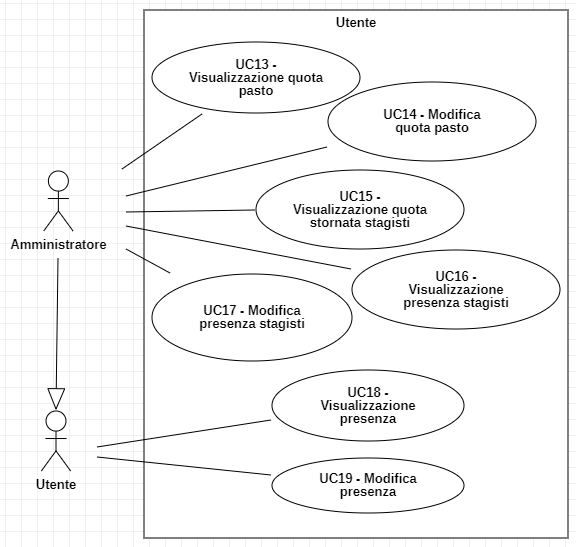
\includegraphics[width=0.9\columnwidth]{usecase/usecase-4} 
    \caption{Use Case - Utente}
    \label{fig:uc-utente}
\end{figure}

\begin{usecase}{13}{Visualizzazione \emph{\gls{quotapastog}}\glsfirstoccur\space - Figura \ref{fig:uc-utente}}
    \usecaseactors{Amministratore}
    \usecasepre{La \emph{\gls{quotapastog}} non è visibile}
    \usecasedesc{L'amministratore entra nell'app per visualizzare la \emph{\gls{quotapastog}}}
    \usecasepost{L'amministratore visualizza la \emph{\gls{quotapastog}}}
    \label{uc:visualizza-quotapasto}
\end{usecase}

\begin{usecase}{14}{Modifica \emph{\gls{quotapastog}} - Figura \ref{fig:uc-utente}}
    \usecaseactors{Amministratore}
    \usecasepre{La \emph{\gls{quotapastog}} è salvata nel database con il vecchio valore}
    \usecasedesc{L'amministratore modifica la \emph{\gls{quotapastog}} con il nuovo valore}
    \usecasepost{La \emph{\gls{quotapastog}} è salvata nel database con il nuovo valore}
    \label{uc:modifica-quotapasto}
\end{usecase}

\begin{usecase}{15}{Visualizzazione \emph{\gls{quotastornatag}} stagisti - Figura \ref{fig:uc-utente}}
    \usecaseactors{Amministratore}
    \usecasepre{La \emph{\gls{quotastornatag}} dei stagisti non è visibile}
    \usecasedesc{L'amministratore entra nell'app per visualizzare la \emph{\gls{quotastornatag}} dei stagisti}
    \usecasepost{L'amministratore visualizza la \emph{\gls{quotastornatag}} dei stagisti}
    \label{uc:visualizza-quotastornatastagisti}
\end{usecase}

\begin{usecase}{16}{Visualizzazione presenza stagisti - Figura \ref{fig:uc-utente}}
    \usecaseactors{Amministratore}
    \usecasepre{La lista delle presenze dei stagisti non è visibile}
    \usecasedesc{L'amministratore entra nell'app per visualizzare la lista delle presenze dei stagisti}
    \usecasepost{L'amministratore visualizza la lista delle presenze dei stagisti}
    \label{uc:visualizza-presenzastagisti}
\end{usecase}

\begin{usecase}{17}{Modifica presenza stagisti - Figura \ref{fig:uc-utente}}
    \usecaseactors{Amministratore}
    \usecasepre{La lista delle presenze dei stagisti è salvata nel database con i vecchi valori}
    \usecasedesc{L'amministratore modifica la lista delle presenze dei stagisti con i nuovi valori}
    \usecasepost{La lista delle presenze dei stagisti è salvata nel database con i nuovi valori}
    \label{uc:modifica-presenzastagisti}
\end{usecase}

\begin{usecase}{18}{Visualizzazione presenza - Figura \ref{fig:uc-utente}}
    \usecaseactors{Utente}
    \usecasepre{La lista delle presenze dell'utente non è visibile}
    \usecasedesc{L'utente entra nell'app per visualizzare la lista delle proprie presenze}
    \usecasepost{L'utente visualizza la lista delle proprie presenze}
    \label{uc:visualizza-presenza}
\end{usecase}

\begin{usecase}{19}{Modifica presenza - Figura \ref{fig:uc-utente}}
    \usecaseactors{Utente}
    \usecasepre{La lista delle presenze dell'utente è salvata nel database con i vecchi valori}
    \usecasedesc{L'utente modifica la lista delle proprie presenze con i nuovi valori}
    \usecasepost{La lista delle presenze dell'utente è salvata nel database con i nuovi valori}
    \label{uc:modifica-presenza}
\end{usecase}

\begin{figure}[!h] 
    \centering 
    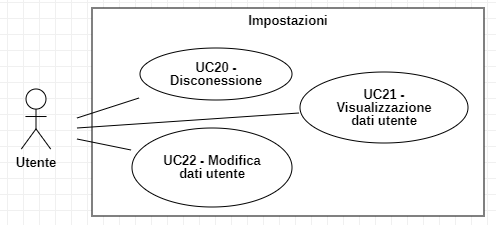
\includegraphics[width=1.0\columnwidth]{usecase/usecase-5} 
    \caption{Use Case - Impostazioni, UC21 e UC22}
    \label{fig:uc-impostazioni}
\end{figure}

\begin{usecase}{20}{Disconnessione - Figura \ref{fig:uc-impostazioni}}
    \usecaseactors{Utente}
    \usecasepre{L'utente è autenticato nell'app}
    \usecasedesc{L'utente si disconnette dalla sessione corrente}
    \usecasepost{L'utente non è autenticato}
    \label{uc:disconnessione-utente}
\end{usecase}

\begin{usecase}{21}{Visualizzazione dati utente - Figura \ref{fig:uc-impostazioni}}
    \usecaseactors{Utente}
    \usecasepre{I dati dell'utente non sono visibili}
    \usecasedesc{L'utente entra nell'app per visualizzare i propri dati}
    \usecasepost{L'utente visualizza i propri dati}
    \label{uc:visualizza-dati}
\end{usecase}

\noindent \textbf{Generalizzazioni:}
\begin{itemize}
    \item \ref{uc:visualizza-mail} - Visualizzazione mail utente
    \item \ref{uc:visualizza-nome} - Visualizzazione nome utente
    \item \ref{uc:visualizza-cognome} - Visualizzazione cognome utente
    \item \ref{uc:visualizza-uid} - Visualizzazione UID Satispay utente
\end{itemize}

\begin{usecase}{21.1}{Visualizzazione mail utente - Figura \ref{fig:uc-impostazioni}}
    \usecaseactors{Utente}
    \usecasepre{La mail dell'utente non è visibile}
    \usecasedesc{L'utente entra nell'app per visualizzare la propria mail}
    \usecasepost{L'utente visualizza la propria mail}
    \label{uc:visualizza-mail}
\end{usecase}

\begin{usecase}{21.2}{Visualizzazione nome utente - Figura \ref{fig:uc-impostazioni}}
    \usecaseactors{Utente}
    \usecasepre{Il nome dell'utente non è visibile}
    \usecasedesc{L'utente entra nell'app per visualizzare il proprio nome}
    \usecasepost{L'utente visualizza il proprio nome}
    \label{uc:visualizza-nome}
\end{usecase}

\begin{usecase}{21.3}{Visualizzazione cognome utente - Figura \ref{fig:uc-impostazioni}}
    \usecaseactors{Utente}
    \usecasepre{Il cognome dell'utente non è visibile}
    \usecasedesc{L'utente entra nell'app per visualizzare il proprio cognome}
    \usecasepost{L'utente visualizza il proprio cognome}
    \label{uc:visualizza-cognome}
\end{usecase}

\newpage

\begin{usecase}{21.4}{Visualizzazione UID Satispay utente - Figura \ref{fig:uc-impostazioni}}
    \usecaseactors{Utente}
    \usecasepre{L'UID Satispay dell'utente non è visibile}
    \usecasedesc{L'utente entra nell'app per visualizzare il proprio UID Satispay}
    \usecasepost{L'utente visualizza il proprio UID Satispay}
    \label{uc:visualizza-uid}
\end{usecase}

\begin{usecase}{22}{Modifica dati utente - Figura \ref{fig:uc-impostazioni}}
    \usecaseactors{Utente}
    \usecasepre{I dati dell'utente sono salvati nel database con i vecchi valori}
    \usecasedesc{L'utente modifica i propri dati con i nuovi valori}
    \usecasepost{I dati dell'utente sono salvati nel database con i nuovi valori}
    \label{uc:modifica-dati}
\end{usecase}

\noindent \textbf{Generalizzazioni:}
\begin{itemize}
    \item \ref{uc:modifica-password} - Modifica password utente
    \item \ref{uc:modifica-nome} - Modifica nome utente
    \item \ref{uc:modifica-cognome} - Modifica cognome utente
    \item \ref{uc:modifica-uid} - Modifica UID Satispay utente
\end{itemize} 

\begin{usecase}{22.1}{Modifica password utente - Figura \ref{fig:uc-impostazioni}}
    \usecaseactors{Utente}
    \usecasepre{La password dell'utente è salvata nel database con il vecchio valore}
    \usecasedesc{L'utente modifica la propria password con il nuovo valore}
    \usecasepost{La password dell'utente è salvata nel database con il nuovo valore}
    \label{uc:modifica-password}
\end{usecase}

\begin{usecase}{22.2}{Modifica nome utente - Figura \ref{fig:uc-impostazioni}}
    \usecaseactors{Utente}
    \usecasepre{Il nome dell'utente è salvato nel database con il vecchio valore}
    \usecasedesc{L'utente modifica il proprio nome con il nuovo valore}
    \usecasepost{Il nome dell'utente è salvato nel database con il nuovo valore}
    \label{uc:modifica-nome}
\end{usecase}

\begin{usecase}{22.3}{Modifica cognome utente - Figura \ref{fig:uc-impostazioni}}
    \usecaseactors{Utente}
    \usecasepre{Il cognome dell'utente è salvato nel database con il vecchio valore}
    \usecasedesc{L'utente modifica il proprio cognome con il nuovo valore}
    \usecasepost{Il cognome dell'utente è salvato nel database con il nuovo valore}
    \label{uc:modifica-cognome}
\end{usecase}

\newpage

\begin{usecase}{22.4}{Modifica UID Satispay utente - Figura \ref{fig:uc-impostazioni}}
    \usecaseactors{Utente}
    \usecasepre{L'UID di Satispay dell'utente è salvato nel database con il vecchio valore}
    \usecasedesc{L'utente modifica il proprio UID Satispay con il nuovo valore}
    \usecasepost{L'UID Satispay dell'utente è salvato nel database con il nuovo valore}
    \label{uc:modifica-uid}
\end{usecase}

\begin{figure}[!h] 
    \centering 
    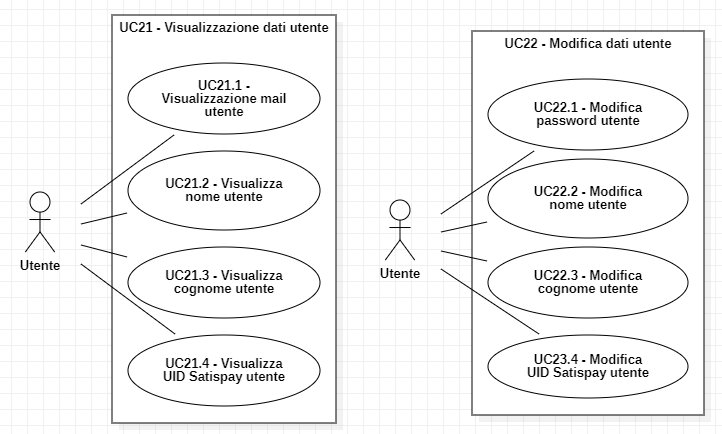
\includegraphics[width=0.7\columnwidth]{usecase/usecase-6} 
    \caption{Use Case - ChatGPT}
    \label{fig:uc-chatgpt}
\end{figure}

\begin{usecase}{23}{Richiesta di una ricetta a ChatGPT - Figura \ref{fig:uc-chatgpt}}
    \usecaseactors{Utente, ChatGPT}
    \usecasepre{L'utente vuole una nuova ricetta}
    \usecasedesc{L'utente chiede a ChatGPT una ricetta}
    \usecasepost{ChatGPT restituisce una possibile ricetta all'utente}
    \label{uc:chatgpt-richiestaricetta}
\end{usecase}

\begin{usecase}{24}{Aggiunta ricetta di ChatGPT nel Menu - Figura \ref{fig:uc-chatgpt}}
    \usecaseactors{Utente}
    \usecasepre{ChatGPT ha consigliato una ricetta all'utente}
    \usecasedesc{L'utente aggiunge la ricetta ricevuta da ChatGPT come nuovo piatto al menu e salva il piatto nel database}
    \usecasepost{La ricetta consigliata da ChatGPT è salvata nel database e visibile dal menu}
    \label{uc:chatgpt-aggiuntaricetta}
\end{usecase}

\newpage

\section{Tracciamento dei requisiti}
\label{sec:requisiti}

Da un'attenta analisi dei requisiti e degli use case effettuata sul progetto è stata stilata la tabella che traccia i requisiti in rapporto agli use case.\\
Sono stati individuati diversi tipi di requisiti e si è quindi fatto utilizzo di un codice identificativo per distinguerli.\\
Il codice dei requisiti è così strutturato R(F/Q/V)(O/D/N) dove:
\begin{enumerate}
	\item[R =] requisito
    \item[F =] funzionale
    \item[Q =] qualitativo
    \item[V =] di vincolo
    \item[O =] obbligatorio (necessario)
    \item[D =] desiderabile
    \item[N =] facoltativo
\end{enumerate}
%Nelle tabelle \ref{tab:requisiti-funzionali}, \ref{tab:requisiti-qualitativi} e \ref{tab:requisiti-vincolo} sono riassunti i requisiti e il loro tracciamento con gli use case delineati in fase di analisi.\newline

%\newpage
%\subsection{Requisiti funzionali}

\begin{table}[htb]%
\caption{Tabella del tracciamento dei requisiti funzionali dall'1 al 7}
\label{tab:requisiti-funzionaliuno}
\begin{tabularx}{\textwidth}{lXl}
\hline
\textbf{Requisito} & \textbf{Descrizione} & \textbf{Use Case}\\
\hline\hline
RFO-1     & L'utente effettua l'accesso all'app inserendo la propria password e la propria mail & UC1 \\
\hline
RFO-2     & L'utente si registra nel database inserendo il proprio nome, cognome, mail e password & UC2 \\
\hline
RFO-3     & Viene visualizzata la \emph{\gls{cassacomuneg}} salvata nel database nell'app & UC3 \\
\hline
RFO-4     & L'utente visualizza la propria \emph{\gls{quotastornatag}} salvata nel database nell'app & UC4 \\
\hline
RFO-5     & Viene visualizzata la lista dei piatti proposti del giorno nell'app & UC5 \\
\hline
RFO-6     & Viene visualizzata la lista delle transazioni nell'app & UC6 \\
\hline
RFO-7     & L'utente aggiunge una nuova transazione nell'app, indicando i soldi e la data e salva la transazione nel database & UC7 \\
\hline
RFO-8     & L'utente amministratore aggiunge la spesa effettuata da uno stagista nell'app, indicando la data e quanto ha speso e lo salva nel database & UC7.1 \\
\hline
RFO-9     & L'utente indica la spesa che ha effettuato nell'app, riportando i soldi e la data e lo salva nel database & UC7.2 \\
\hline
RFO-10    & L'utente indica nell'app i soldi che ha inviato a un altro utente registrato nel database e salva la transazione nel database & UC7.3 \\
\hline
RFO-11    & L'utente elimina una transazione presente nel database dall'app & UC8 \\
\hline
RFO-12    & Viene visualizzato il menu che contiene la lista dei piatti dall'app & UC9 \\
\hline
\end{tabularx}
\end{table}%

\begin{table}%
\caption{Tabella del tracciamento dei requisiti funzionali dall'8 al 31}
\label{tab:requisiti-funzionalidue}
\begin{tabularx}{\textwidth}{lXl}
\hline
\textbf{Requisito} & \textbf{Descrizione} & \textbf{Use Case}\\
\hline\hline
RFO-13    & L'utente aggiunge un nuovo piatto nell'app, indicando il nome del piatto, gli ingredienti e la ricetta e lo salva nel database & UC10 \\
\hline
RFO-14    & L'utente elimina un piatto presente nel database dall'app & UC11 \\
\hline
RFO-15    & L'utente propone un piatto da mangiare a pranzo selezionandolo dal menu & UC12 \\
\hline
RFO-16    & L'amministratore visualizza la \emph{\gls{quotapastog}} dall'app & UC13 \\
\hline
RFO-17    & L'amministratore modifica la \emph{\gls{quotapastog}} dall'app e salva il nuovo valore nel database & UC14 \\
\hline
RFO-18    & L'amministratore visualizza la \emph{\gls{quotastornatag}} degli stagisti dall'app & UC15 \\
\hline
RFO-19    & L'amministratore visualizza la lista con indicato i giorni di presenza degli stagisti dall'app & UC16 \\
\hline
RFO-20    & L'amministratore modifica la lista con indicato i giorni di presenza degli stagisti dall'app e salva le modifiche nel database & UC17 \\
\hline
RFO-21    & L'utente visualizza la lista con indicati i propri giorni di presenza a pranzo dall'app & UC18 \\
\hline
RFO-22    & L'utente modifica la lista con indicati i propri giorni di presenza a pranzo dall'app e salva le modifiche nel database & UC19 \\
\hline
RFO-23    & L'utente si disconnette dall'app & UC20 \\
\hline
RFO-24    & L'utente visualizza i propri dati dall'app & UC21 \\
\hline
RFO-25    & L'utente visualizza la propria mail dall'app & UC21.1 \\
\hline
RFO-26    & L'utente visualizza il proprio nome dall'app & UC21.2 \\
\hline
RFO-27    & L'utente visualizza il proprio cognome dall'app & UC21.3 \\
\hline
RFO-28    & L'utente visualizza il proprio UID Satispay dall'app & UC21.4 \\
\hline
RFO-29    & L'utente modifica i propri dati dall'app e salva le modifiche nel database & UC22 \\
\hline
RFO-30    & L'utente modifica la propria password dall'app e salva la nuova password nel database & UC22.1 \\
\hline
RFO-31    & L'utente modifica il proprio nome dall'app e salva il nuovo nome nel database & UC22.2 \\
\hline
RFO-32    & L'utente modifica il proprio cognome dall'app e salva il nuovo cognome nel database & UC22.3 \\
\hline
RFO-33    & L'utente modifica il proprio UID Satispay e salva il nuovo UID nel database & UC22.4 \\
\hline
RFD-34    & Viene chiesto a ChatGPT una possibile ricetta da proporre a pranzo & UC23 \\
\hline
RFD-35    & Si aggiunge la ricetta proposta da ChatGPT nel menu e si salva la ricetta nel database & UC24 \\
\hline
\end{tabularx}
\end{table}%

\newpage

%\subsection{Requisiti qualitativi}

\begin{table}[htb]%
\caption{Tabella del tracciamento dei requisiti qualitativi}
\label{tab:requisiti-qualitativi}
\begin{tabularx}{\textwidth}{lXl}
\hline
\textbf{Requisito} & \textbf{Descrizione} & \textbf{Use Case}\\
\hline\hline
RQN-1    & Il codice \emph{front-end} deve essere coperto da test di unità & - \\
\hline
\end{tabularx}
\end{table}%

%\subsection{Requisiti di vincolo}

\begin{table}[htb]%
\caption{Tabella del tracciamento dei requisiti di vincolo}
\label{tab:requisiti-vincolo}
\begin{tabularx}{\textwidth}{lXl}
\hline
\textbf{Requisito} & \textbf{Descrizione} & \textbf{Use Case}\\
\hline\hline
RVO-1    & L'applicazione deve essere sviluppata con il \emph{framework} Flutter & - \\
\hline
RVO-2    & L'applicazione deve essere sviluppata con la piattaforma Firebase & - \\
\hline
RVO-3    & L'applicazione deve essere accessibile su cellulari con sistema operativo Android e iOS & - \\
\hline
RVO-4    & La mail che l'utente deve utilizzare per registrarsi nel database e accedere all'app deve essere fornita da RiskAPP & - \\
\hline
RVO-5    & La mail dell'utente non deve essere modificabile tramite app & - \\
\hline
\end{tabularx}
\end{table}%
